\documentclass[12pt]{article}

\usepackage[english]{babel}
\usepackage[utf8]{inputenc}
\usepackage[top=2cm, left=2cm, right=2cm, bottom=2cm]{geometry}
\usepackage[document]{ragged2e}
\usepackage{tikz,minted,times}

\setlength\parindent{0pt}
\sloppy
\usetikzlibrary{automata,positioning,arrows}
\tikzset{node distance=2.5cm,every state/.style={semithick,fill=gray!10},initial text={},double distance=2pt,every edge/.style={draw,->,>=stealth,auto,semithick}}
\usemintedstyle{colorful}

\title{COMP SCI 7411 Event Driven Computing Practice 1 Plan}
\author{Tinson Lai \\ a1812422}
\date{\today}

\begin{document}

\maketitle

\section{Locking}

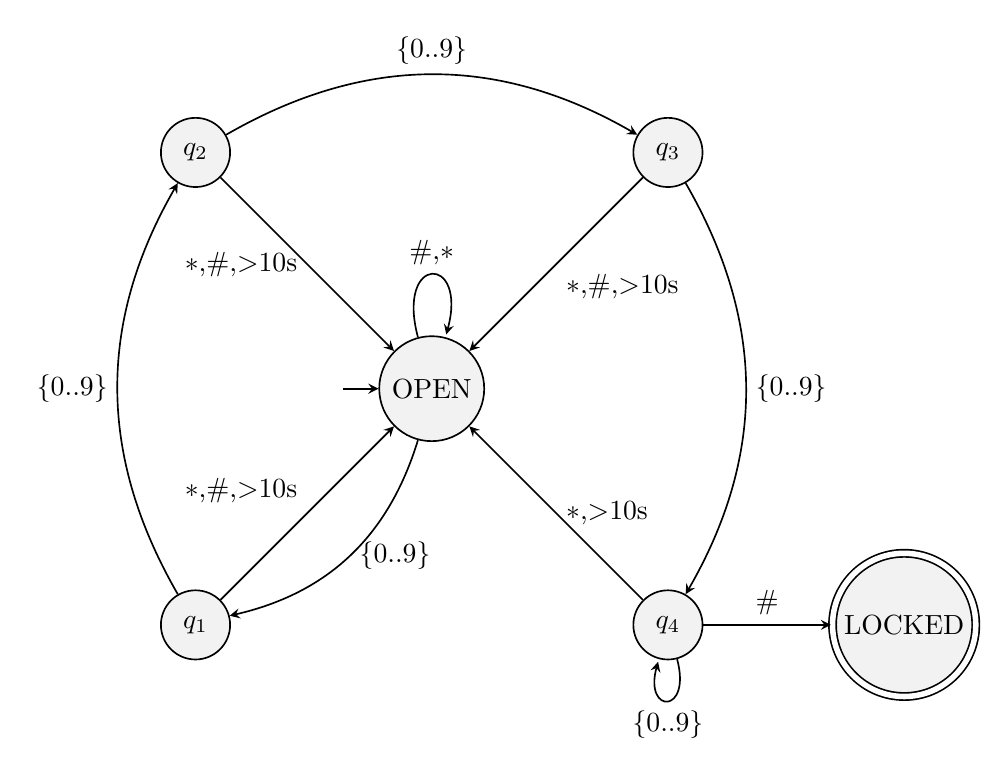
\begin{tikzpicture}
  \node[state, initial] at (3, 3) (open){OPEN};
  \node[state] at (0, 0) (q1){$q_1$};
  \node[state] at (0, 6) (q2){$q_2$};
  \node[state] at (6, 6) (q3){$q_3$};
  \node[state] at (6, 0) (q4){$q_4$};
  \node[state, accepting] at (9, 0) (locked){LOCKED};

  \draw

  (open) edge[loop above] node{$\#$,$*$} (open)
  (open) edge[bend left, right] node{$\left\{0..9\right\}$} (q1)
  (q1) edge[bend left, left] node{$\left\{0..9\right\}$} (q2)
  (q2) edge[bend left, above] node{$\left\{0..9\right\}$} (q3)
  (q3) edge[bend left, right] node{$\left\{0..9\right\}$} (q4)
  (q4) edge[loop below, below] node{$\left\{0..9\right\}$} (q4)

  (q1) edge node{$*$,$\#$,$>$10s} (open)
  (q2) edge[left] node{$*$,$\#$,$>$10s} (open)
  (q3) edge node{$*$,$\#$,$>$10s} (open)
  (q4) edge node{$\#$} (locked)
  (q4) edge[right] node{$*$,$>$10s} (open)

  ;
\end{tikzpicture}

The design above has several notations which might be unclear:
\begin{itemize}
  \item State is named $q_i$ where $i$ represents the number of digits shown in the panel display.
  \item $>$10s means the timer has recorded a duration longer than 10 seconds. Notice that the timer is started in state $q_1$, and will be reset in both OPEN and LOCKED states.
  \item $\#$ means presssing the key $\#$ once, similar for $*$. $\left\{0..9\right\}$ means pressing one of the numeric keys on the panel once.
\end{itemize}

\section{Unlocking}

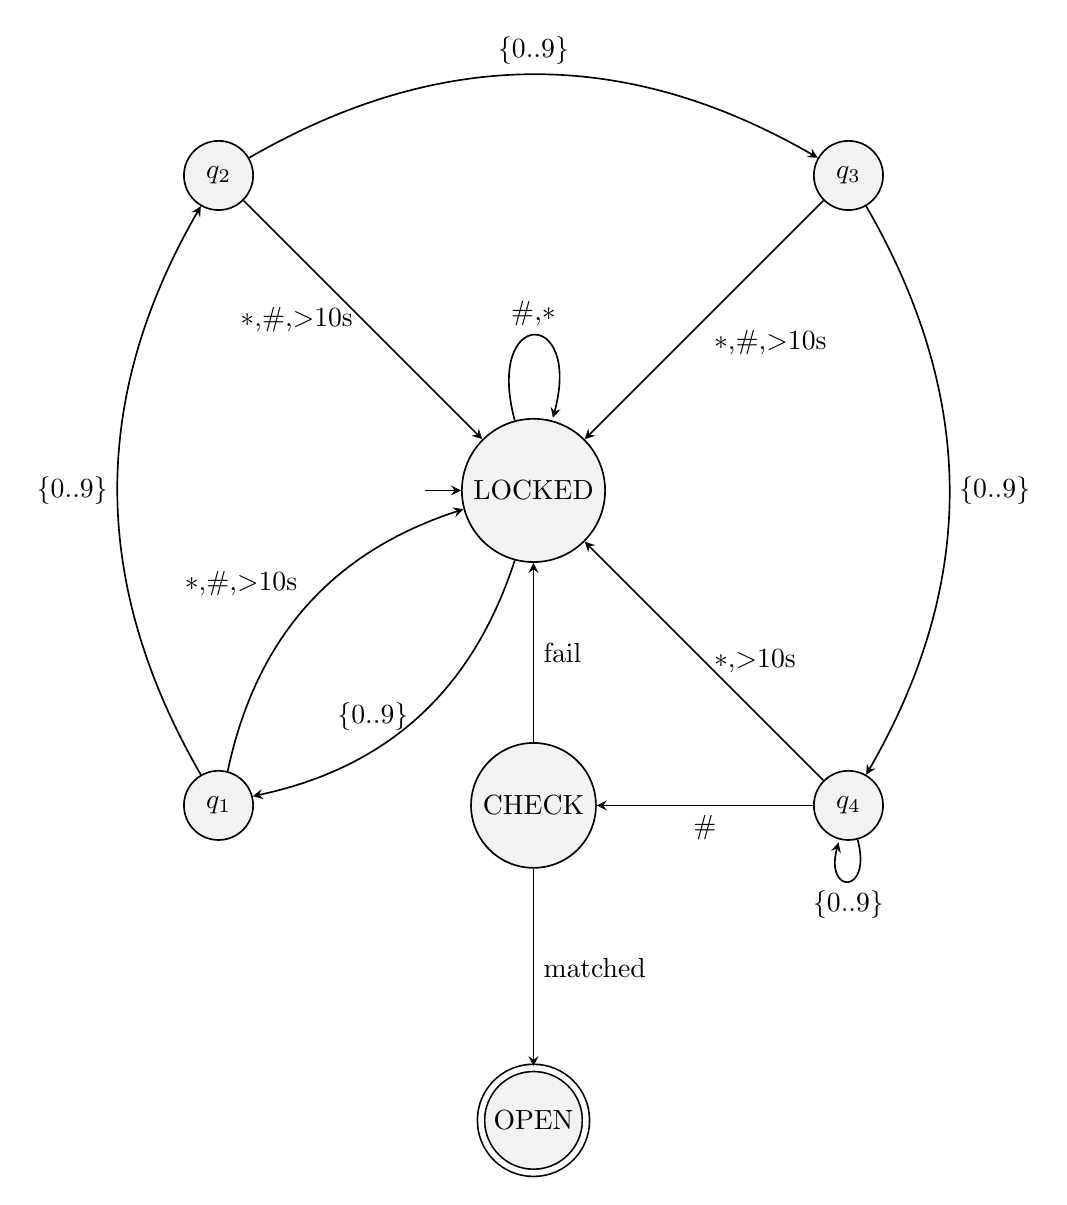
\begin{tikzpicture}
  \node[state, initial] at (4, 8) (locked){LOCKED};
  \node[state] at (0, 4) (q1){$q_1$};
  \node[state] at (0, 12) (q2){$q_2$};
  \node[state] at (8, 12) (q3){$q_3$};
  \node[state] at (8, 4) (q4){$q_4$};
  \node[state] at (4, 4) (check){CHECK};
  \node[state, accepting] at (4, 0) (open){OPEN};

  \draw

  (locked) edge[loop above] node{$\#$,$*$} (locked)
  (locked) edge[bend left, left] node{$\left\{0..9\right\}$} (q1)
  (q1) edge[bend left, left] node{$\left\{0..9\right\}$} (q2)
  (q2) edge[bend left, above] node{$\left\{0..9\right\}$} (q3)
  (q3) edge[bend left, right] node{$\left\{0..9\right\}$} (q4)
  (q4) edge[loop below, below] node{$\left\{0..9\right\}$} (q4)

  (q1) edge[bend left] node{$*$,$\#$,$>$10s} (locked)
  (q2) edge[left] node{$*$,$\#$,$>$10s} (locked)
  (q3) edge node{$*$,$\#$,$>$10s} (locked)
  (q4) edge node{$\#$} (check)
  (q4) edge[right] node{$*$,$>$10s} (locked)

  (check) edge[right] node{fail} (locked)
  (check) edge node{matched} (open)

  ;
\end{tikzpicture}

The notations here are the same as the previous graph, and these two graphs are quite similar as well. The CHECK state is an intermediate state used to represent the process of password checking.

\section{Timer}

The timer used in the previous two graphs has a simpler state diagram.

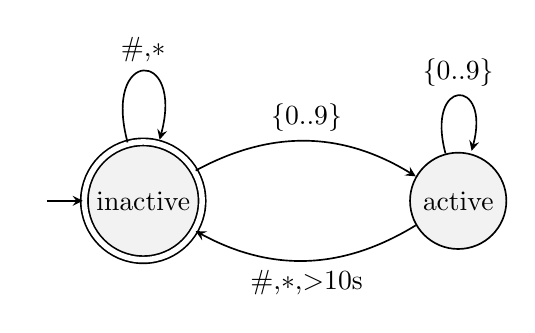
\begin{tikzpicture}
  \node[state, initial, accepting] at (0, 0) (inactive){inactive};
  \node[state] at (4, 0) (active){active};

  \draw

  (inactive) edge[loop above] node{$\#$,$*$} (inactive)
  (inactive) edge[bend left] node{$\left\{0..9\right\}$} (active)
  (active) edge[loop above] node{$\left\{0..9\right\}$} (active)
  (active) edge[bend left] node{$\#$,$*$,$>$10s} (inactive)

  ;
\end{tikzpicture}

\section{Extra}

\begin{itemize}
  \item Although $\#$ and $*$ seems to be identical in the state diagram in the state diagram, in real world, this will usually be just a beep sound played by the lock if someone entered an incorrect password. In the implementation, however, the effect will be just clearing the input box as it returns back to the starting state.
  \item The design choice of the transition from $q_4$ looping back to $q_4$ is based on most of the common real-world appliances. All redundant number pressed after the input box is full will be discarded automatically.
\end{itemize}

\end{document}
